\chapter[The CMS at the LHC]{The CMS at the LHC}

This chapter will provide an overview of the European Organization for Nuclear Research, commonly known by its acronym CERN (Conseil Européen pour la Recherche Nucléaire), along with the Large Hadron Collider (LHC) and the Compact Muon Solenoid (CMS) experiment. It will go through the most significant breakthroughs at CERN, with a particular emphasis on the discovery of the Higgs boson at the LHC in 2012 by the CMS and ATLAS collaborations \cite{CMS:2012qbp,ATLAS:2012yve}.

\section{The Large Hadron Collider at CERN}

The European Organization for Nuclear Research (CERN) is an intergovernmental organization composed of 23 member states that operates the world's largest particle physics laboratory. Established in 1954, CERN is situated on the Franco-Swiss border near Geneva, Switzerland, and is one of the largest and most influential research organizations in particle physics. The missions of CERN include world-class research in fundamental physics, sustainable and environmentally responsible accelerator facilities, global collaboration in science and technology advancement and the education and engagement of future scientists, engineers and the broader public.

CERN has been home to many accelerators, including the original linear accelerator \linebreak LINAC 1 (in operation from 1959 until 1992), the LINAC 2 (1978 - 2018), the Super Proton-Antiproton Synchrotron (S$p\bar{p}$S) (1981-1991), the Large Electron-Positron Collider (LEP) (1989-2000), and the current Large Hadron Collider (LHC), which was constructed between 1998 and 2008 and achieved its first collisions in 2010. The Future Circular Collider (FCC) is proposed to be the successor of LHC at CERN \cite{FCC:2018byv}.

During its nearly 70-year history since its creation, many important achievements in particle physics have been made through experiments at CERN, including:
\begin{itemize}
    \setlength\itemsep{0em}
    \item The discovery of neutral currents by studying neutrinos produced by the PS/SPS neutrino beam interacting in the Gargamelle bubble chamber in 1973 \cite{GargamelleNeutrino:1973jyy}.
    \item The discovery of the $W^\pm$ and $Z^0$ bosons in the UA1 and UA2 experiments in 1983 \cite{UA1:1983crd, UA2:1983tsx}.
    \item The determination of the number of light neutrino families at LEP in 1989 \cite{ALEPH:1989kcj}.
    \item The discovery of direct CP violation in the NA48 experiment in 1999 \cite{NA48:1999szy}.
    \item The discovery of the Higgs boson at LHC by the CMS and ATLAS collaborations in 2012 \cite{CMS:2012qbp,ATLAS:2012yve}.
\end{itemize}

The Large Hadron Collider (LHC) at CERN is a hadron collider primarily used for proton-proton collisions, but also capable of heavy-ion collisions. It has a circumference of 26.659 kilometers and is located underground at depths ranging from 50 to 175 meters, making it the world's largest and highest-energy particle collider \cite{Evans:2008zzb, CERN:Facts_figures}.

\begin{figure}[!ht]
    \vspace*{-0.0cm}
    \centering
    \setlength{\mylength}{\textwidth}
    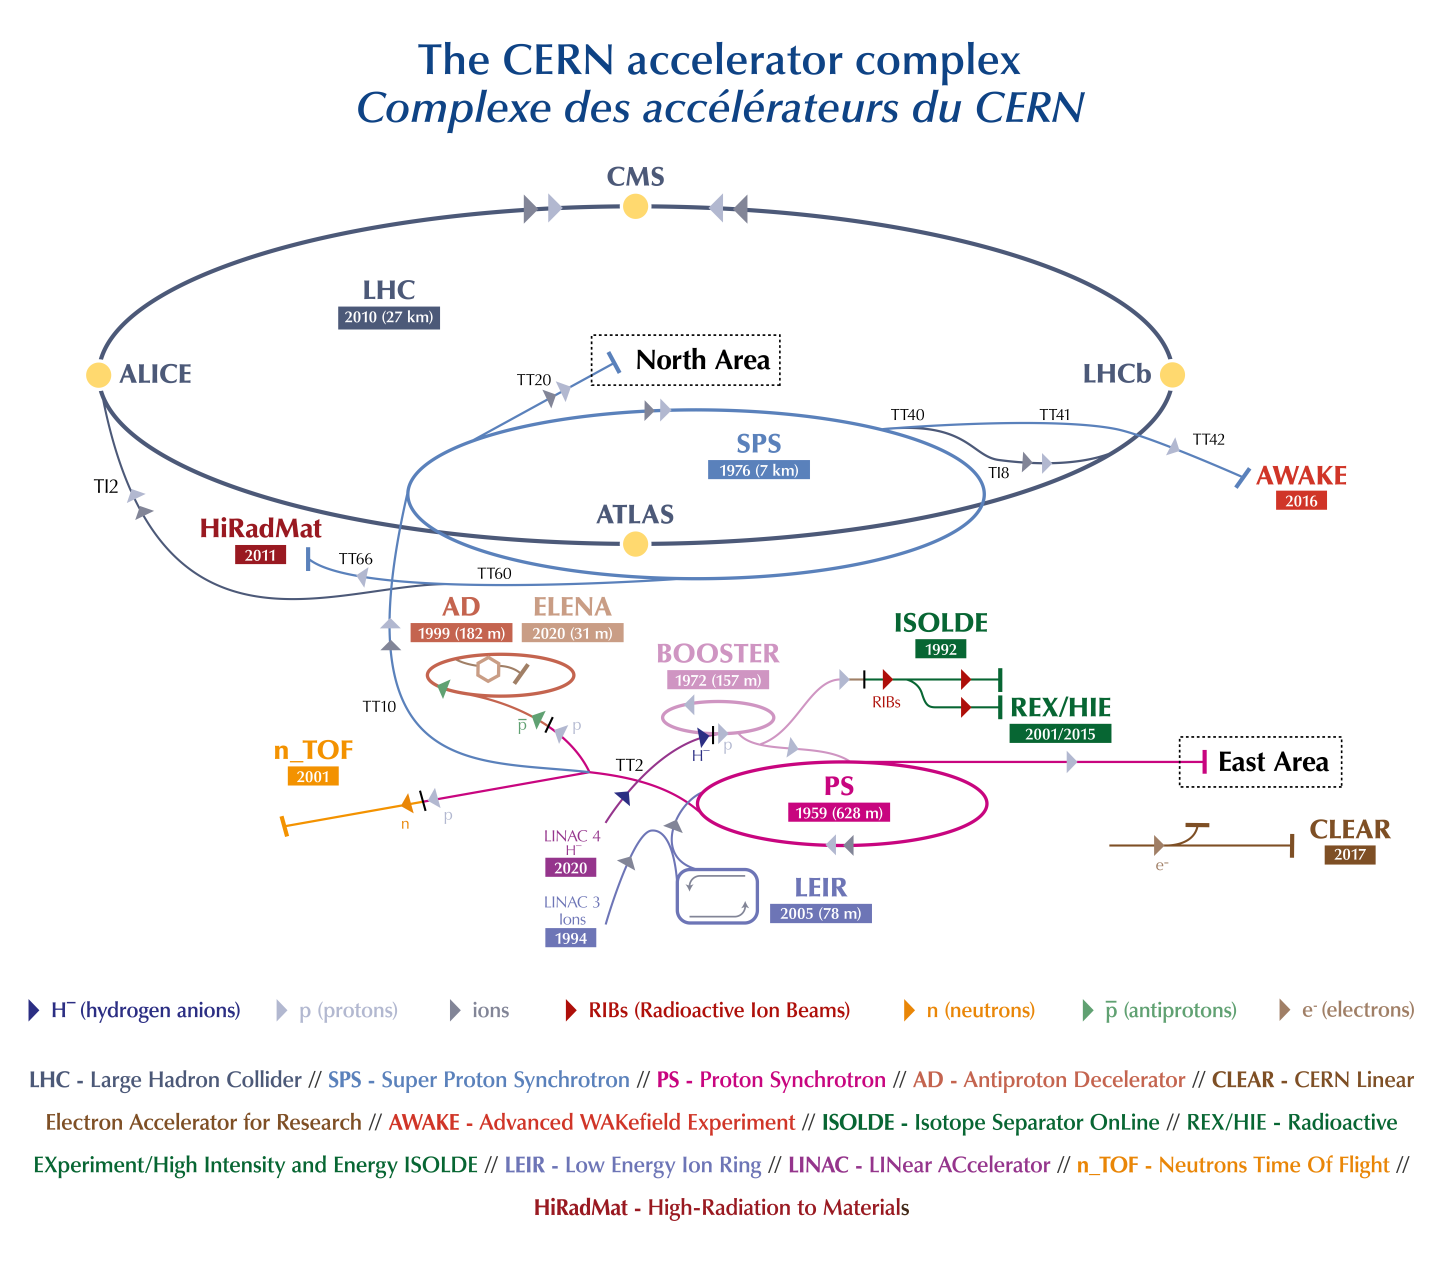
\includegraphics[width=0.84\mylength]{resources/LHC.png}
    \vspace*{-0.0cm}
    \caption{The CERN accelerator complex. The four main experiments can be seen in four different points around the LHC. Source: \cite{Mobs:2684277}.}
    \label{fig:CERN_LHC}
    \vspace*{-0.3cm}
\end{figure}

There are two beams going in opposite directions within the LHC, which are bent and focused by 9593 superconducting magnets. At a center-of-mass energy of $\sqrt{s} = 13\ \TeV$, protons from each beam have an energy of 6.5 TeV and complete approximately 11245 orbits around the collider's circumference every second. There are 2808 bunches per proton beam, resulting in collisions approximately every 25 ns, equivalent to a frequency of 40 MHz. These collisions take place at four interaction points where the four major LHC experiments are positioned:  ATLAS (A Toroidal LHC ApparatuS) \cite{ATLAS:1994vge}, CMS (Compact Muon Solenoid) \cite{CMS:1994hea}, ALICE (A Large Ion Collider Experiment) \cite{413235}, and LHCb (Large Hadron Collider beauty) \cite{LHCb:1998kcv}. Among these four experiments, ATLAS and CMS are multipurpose detectors designed to study a wide range of physics phenomena. ALICE is specifically conceived to record the collisions of ion beams, while LHCb is designed to optimally study $b$-physics. Moreover, several smaller experiments at the LHC focus on more specific physics goals. A diagram of CERN's Accelerator Complex is shown in Figure \ref{fig:CERN_LHC}.

During Run 1 of the LHC, which spanned from 2010 to 2012, the center-of-mass energy ranged from 7 to 8 TeV, and CMS recorded a total integrated luminosity of 29.45 fb$^{-1}$. Run 2 took place from 2015 to 2018, with an energy of 13 TeV, and a total integrated luminosity of 163.6 fb$^{-1}$. In 2022, Run 3 began and is scheduled to conclude in 2026, with an energy of 13.6 TeV. In the first year of Run 3, the total integrated luminosity reached 42 fb$^{-1}$, and is expected to be around 300 by the end of the Run \cite{CMS:luminosity}. The data that is going to be used in this analysis is from the CMS collaboration and was taken in 2018 (Run 2), with $\sqrt{s} = 13\ \TeV$ and an integrated luminosity of 39.5 fb$^{-1}$.

\section{The Compact Muon Solenoid}

\todo{What is the CMS collaboration?}

\todo{explain the detector}

\todo{mention discoveries and relevant papers}

\todo{1 paragraph about computer facilities and clusters (T0, T1...)}

\section{The discovery of the Higgs boson at CMS}

\todo{Discovery of the higgs: when, CMS/ATLAS, which channels were used, sigmas, initial mass and values.}

